\section{Modelo de Arquitectura}

El diseño arquitectónico de la plataforma se fundamenta en un enfoque híbrido que combina la escalabilidad de los microservicios con la robustez del patrón de diseño de tres capas. Esta decisión técnica garantiza la independencia operativa de los módulos de gestión administrativa y de inteligencia artificial, asegurando la mantenibilidad a largo plazo del sistema.

\subsection{Visión General de la Arquitectura de Microservicios}

La arquitectura de la plataforma se fundamenta en la descomposición del sistema en servicios pequeños, autónomos y altamente cohesivos que se comunican a través de protocolos ligeros (REST/JSON). Esta decisión técnica permite que cada unidad funcional del sistema de la Defensoría opere como un proceso independiente, facilitando su despliegue, mantenimiento y escalabilidad de forma aislada.

\subsubsection*{Racionalidad de la Descomposición Funcional}
A diferencia de un modelo monolítico tradicional, donde una falla en el módulo de procesamiento de texto podría comprometer la gestión completa de expedientes, esta arquitectura garantiza la resiliencia operativa. El sistema se divide estratégicamente en dos dominios tecnológicos:

\begin{itemize}
    \item \textbf{Núcleo Administrativo y de Gestión:} Desarrollado en Java con el framework Spring Boot. Se encarga de la persistencia de datos, gestión de flujos de trabajo legales, control de acceso basado en roles (RBAC) y la generación de documentos oficiales.
    \item \textbf{Módulo de Inteligencia Artificial:} Implementado en Python mediante FastAPI. Especializado en el Procesamiento de Lenguaje Natural (PLN) para la determinación automática de competencia basada en el análisis semántico de las denuncias.
\end{itemize}

\subsubsection*{Heterogeneidad Tecnológica y Especialización}
La arquitectura permite la coexistencia de tecnologías heterogéneas, seleccionando el lenguaje más apto para cada necesidad específica del proyecto:
\begin{enumerate}
    \item \textbf{Java (JVM):} Proporciona un tipado estricto y una gestión de memoria robusta, ideal para la lógica de negocio crítica y la seguridad de los datos personales en cumplimiento con la normativa institucional.
    \item \textbf{Python:} Ofrece acceso al estado del arte en aprendizaje automático, facilitando la integración de modelos de \textit{Embeddings} y transformadores para capturar matices semánticos en las narrativas de los quejosos.
\end{enumerate}

\begin{figure}[htbp]
    \centering
    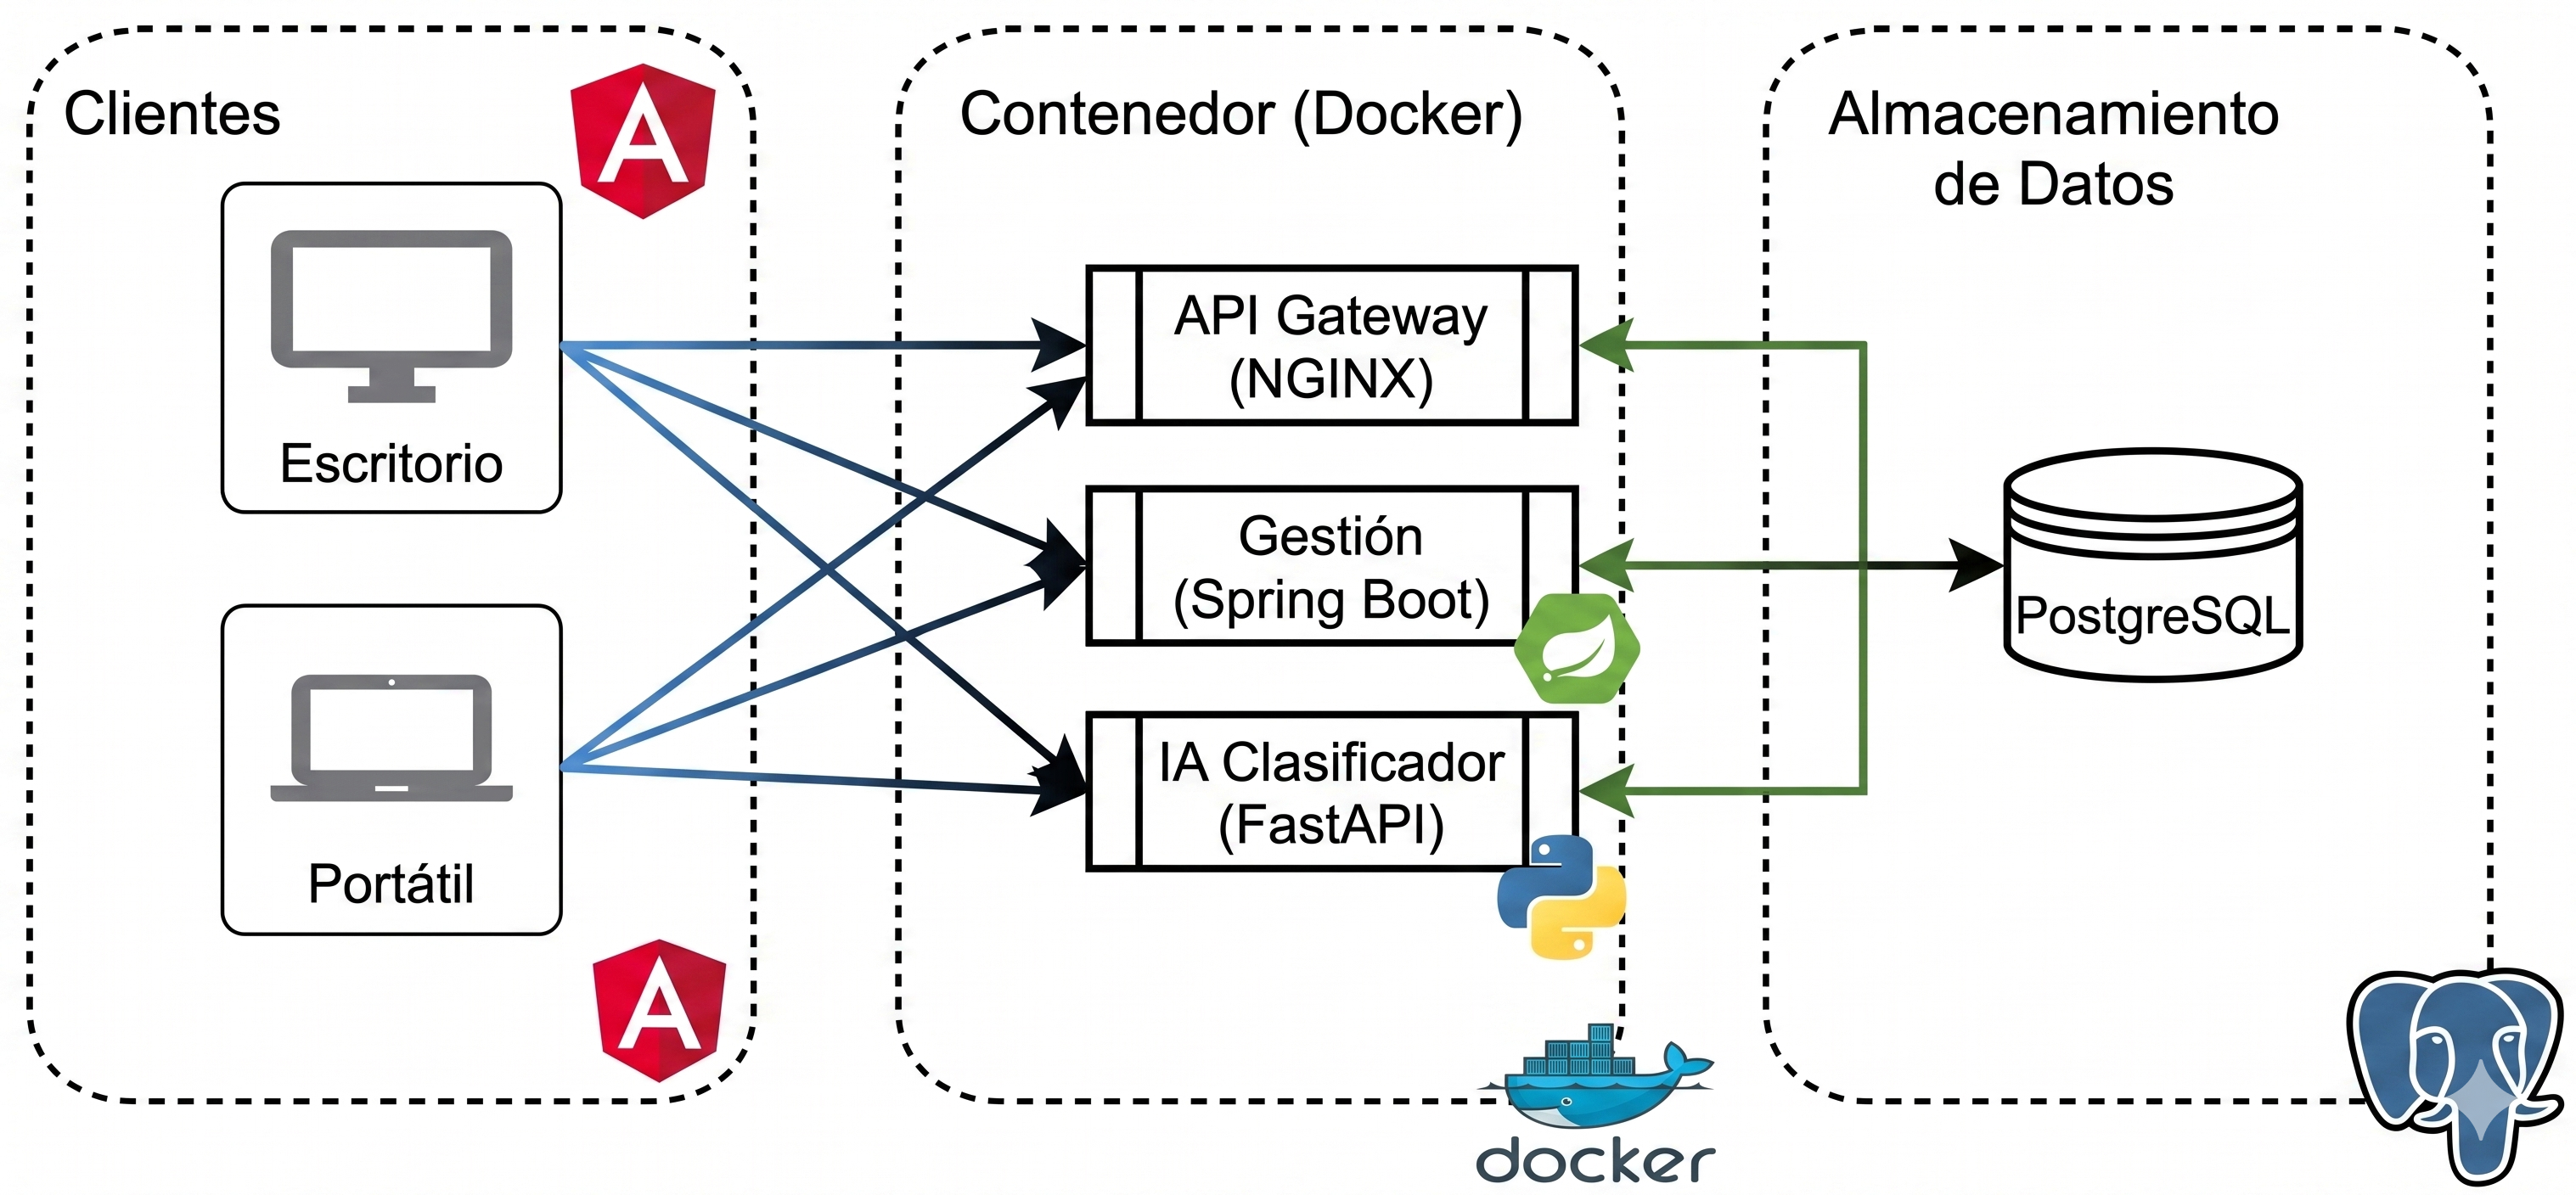
\includegraphics[width=0.8\textwidth]{imagenes/documento/diagrama_microservicios.png}
    \caption{Esquema conceptual de la comunicación entre el API Gateway, los microservicios de gestión (Java) y el clasificador (Python).}
    \label{fig:arquitectura_overview}
\end{figure}

\subsubsection*{Beneficios para la Defensoría de los Derechos Politécnicos}
La implementación de este esquema arquitectónico ofrece ventajas estratégicas alineadas con los objetivos del Trabajo Terminal:
\begin{itemize}
    \item \textbf{Escalabilidad Granular:} Es posible asignar recursos adicionales exclusivamente al microservicio de IA durante periodos de alta demanda de denuncias.
    \item \textbf{Aislamiento de Fallos:} Una saturación en el motor de clasificación no impide que el personal administrativo continúe con la integración de expedientes ya radicados.
    \item \textbf{Interoperabilidad:} El uso de un API Gateway centraliza el tráfico y estandariza la seguridad mediante protocolos TLS 1.3, protegiendo la información sensible en tránsito.
\end{itemize}


\subsection{Arquitectura Interna: Patrón de 3 Capas}

Cada microservicio que integra la plataforma implementa internamente una estructura de tres niveles lógicos, cuyo objetivo primordial es garantizar el desacoplamiento de responsabilidades y facilitar la mantenibilidad del sistema a largo plazo. Este diseño permite que la lógica institucional de la Defensoría permanezca aislada de las interfaces de usuario y de los motores de persistencia físicos .

\begin{figure}[htbp]
    \centering
    % Imagen general que muestra las 3 capas unidas
    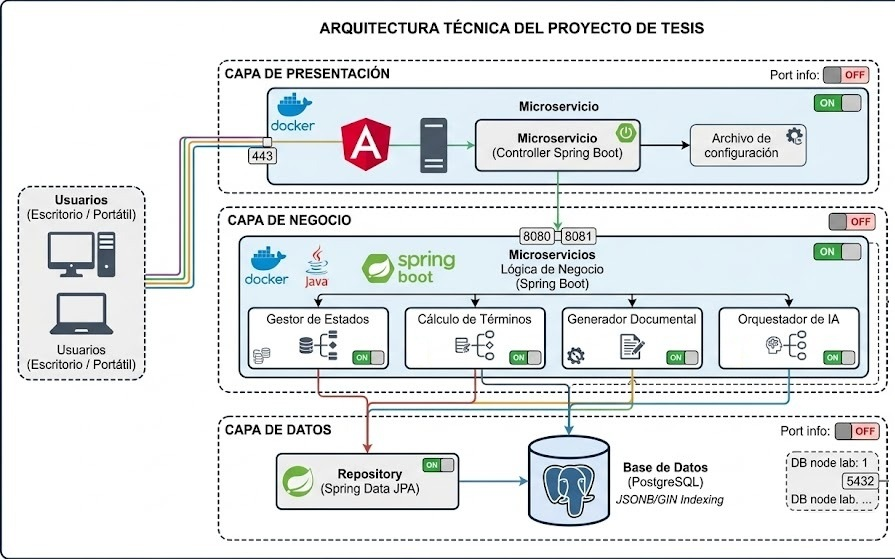
\includegraphics[width=0.85\textwidth]{imagenes/documento/arquitectura_interna_general.png}
    \caption{Diagrama de arquitectura interna detallando la interacción entre los niveles de presentación, negocio y datos.}
    \label{fig:arquitectura_interna_3capas}
\end{figure}

\subsubsection{Capa de Presentación (Interfaz y Controladores)}

Esta capa constituye el nivel más externo del microservicio y actúa como la frontera de comunicación con el exterior. Su responsabilidad principal es capturar las peticiones de los usuarios y presentar los resultados de forma estructurada .

\begin{itemize}
    \item \textbf{Interfaz de Usuario (Angular):} Gestiona la interacción reactiva con el quejoso y el personal de la DDP. Utiliza servicios inyectables para realizar peticiones asíncronas hacia el backend, manejando estados de carga y errores de red en tiempo real.
    \item \textbf{Controladores REST (Spring Boot / FastAPI):} Representan los \textit{endpoints} de la API. Se encargan de la validación sintáctica de entrada (formatos de archivos, tipos de datos) y de la serialización de los objetos de negocio a formato JSON para su transmisión.
\end{itemize}


\subsubsection{Capa de Lógica de Negocio (Service Layer)}

Considerada el núcleo o cerebro del sistema, esta capa es donde se codifican rigurosamente las reglas institucionales y los flujos operativos definidos en el Manual de Procedimientos de la Defensoría .

\begin{itemize}
    \item \textbf{Gestor de Ciclo de Vida:} Controla la transición de estados de las quejas (Recibida, En Revisión, Concluida), asegurando que cada paso cumpla con las precondiciones normativas antes de avanzar.
    \item \textbf{Monitoreo de Términos Procesales:} Implementa algoritmos para el cálculo automático de plazos legales (de 2 a 15 días hábiles), generando alertas preventivas ante posibles rezagos administrativos.
    \item \textbf{Orquestación del Clasificador:} Coordina la comunicación con el microservicio especializado en PLN, enviando la narrativa de los hechos para obtener una sugerencia de competencia basada en el Artículo 4º del reglamento.
\end{itemize}



\subsubsection{Capa de Persistencia (Acceso a Datos)}

Responsable de la comunicación directa con el motor de base de datos PostgreSQL, garantizando que la información de la comunidad politécnica sea duradera y se encuentre segura en reposo .

\begin{itemize}
    \item \textbf{Patrón Repository:} Implementa una capa de abstracción mediante Spring Data JPA, eliminando el uso de consultas SQL manuales y protegiendo al sistema contra ataques de inyección de código.
    \item \textbf{Gestión de Datos Semi-estructurados:} Utiliza el tipo de dato \texttt{JSONB} para el almacenamiento flexible de metadatos de evidencias digitales y emplea índices \texttt{GIN} para búsquedas semánticas rápidas.
    \item \textbf{Repositorio de Evidencias:} Gestiona la persistencia física de documentos (PDF) y archivos multimedia, asegurando la integridad de los expedientes digitales mediante identificadores únicos vinculados a cada folio.
\end{itemize}


\subsection{Infraestructura y Seguridad de la Arquitectura}

La robustez de la plataforma se sustenta en una infraestructura diseñada bajo estándares modernos de ciberseguridad y escalabilidad, garantizando que la transición hacia la gestión digital de quejas en la Defensoría se realice de forma segura y eficiente .

\subsubsection{Comunicación y Gateway}

Para la gestión del tráfico externo y la protección de los servicios internos, se implementó el patrón \textbf{API Gateway} utilizando \textbf{NGINX} como servidor de entrada único. Este componente actúa como la frontera de seguridad perimetral del sistema, abstrayendo la complejidad de la arquitectura de microservicios .

\begin{itemize}
    \item \textbf{Cifrado en Tránsito mediante TLS 1.3:} La seguridad de las comunicaciones entre los quejosos y el servidor institucional se garantiza mediante el protocolo \textbf{TLS 1.3}. Esta implementación asegura que el intercambio de información sensible, como evidencias y narrativas jurídicas, viaje cifrado de extremo a extremo, protegiendo la integridad del expediente digital frente a intercepciones no autorizadas.
    \item \textbf{Seguridad Perimetral y Control de Acceso:} El Gateway centraliza la validación de tokens \textbf{JWT (JSON Web Tokens)}. Mediante esta estrategia, el sistema intercepta cada petición HTTP para verificar la autenticidad del usuario y validar sus permisos según el modelo \textbf{RBAC} (Control de Acceso Basado en Roles) antes de permitir la interacción con la lógica de negocio en Java o Python.
\end{itemize}

\subsubsection{Contenerización y Orquestación}

La plataforma adopta la tecnología de contenerización para mitigar los riesgos derivados de la heterogeneidad tecnológica y asegurar la portabilidad del sistema entre diferentes entornos de ejecución .

\begin{itemize}
    \item \textbf{Empaquetado con Docker:} Cada unidad funcional (Presentación, Negocio y Datos) ha sido encapsulada en contenedores autónomos de \textbf{Docker}. Este enfoque permite que el microservicio de gestión en \textbf{Spring Boot} y el clasificador de IA en \textbf{FastAPI} coexistan de manera aislada, incluyendo todas sus dependencias y sistemas de archivos específicos dentro de una imagen inmutable.
    \item \textbf{Gestión mediante Docker Compose:} La orquestación del despliegue se realiza a través de \textbf{Docker Compose}, lo que permite definir la infraestructura como código. Esta herramienta gestiona la interconexión de redes internas entre contenedores y automatiza la persistencia de la base de datos \textbf{PostgreSQL}, asegurando que el sistema pueda ser replicado fielmente en el servidor institucional con un esfuerzo de configuración mínimo.
    \item \textbf{Aislamiento de Recursos y Disponibilidad:} Al operar en contenedores separados, se garantiza que un fallo crítico o una saturación de memoria en un módulo específico no comprometa la estabilidad global de la plataforma, permitiendo el mantenimiento independiente de cada componente sin interrumpir el servicio a la comunidad politécnica.
\end{itemize}